% S2880814 MSc Dissertation
% Built from the infthesis skeleton, populated with content ported from the
% dissertation progress report (S2880814_Dissertation_Progress_Report/main.tex).
%
% \documentclass[logo,msc,adi]{infthesis}     % Adv Design Inf
\documentclass[logo,msc,ai]{infthesis}        % AI
% \documentclass[logo,msc,cogsci]{infthesis}  % Cognitive Sci
% \documentclass[logo,msc,cs]{infthesis}      % Computer Sci
% \documentclass[logo,msc,cyber]{infthesis}   % Cyber Sec
% \documentclass[logo,msc,datasci]{infthesis} % Data Sci
% \documentclass[logo,msc,di]{infthesis}      % Design Inf
% \documentclass[logo,msc,dsti]{infthesis}    % Data Sci TI
% \documentclass[logo,msc,inf]{infthesis}     % Informatics
%%%%%%%%%%%%%%%%%%%%%%%%
\usepackage{msccheck}

% Content packages only; none of these change page layout, margins, or
% line spacing (see msccheck.sty, which checks exactly that).
\usepackage[utf8]{inputenc}
\usepackage[T1]{fontenc}
\usepackage{microtype}
\usepackage{graphicx}
\usepackage{booktabs}
\usepackage{array}
\usepackage{longtable}
\usepackage{ragged2e}
\usepackage{xcolor}
\usepackage{pgfgantt}
\usepackage{hyperref}

% Custom ragged-right fixed-width column type, used throughout the result tables.
\newcolumntype{L}[1]{>{\RaggedRight\arraybackslash}p{#1}}

% Colours used only inside the Gantt chart figure in Chapter~\ref{sec:plan}.
\definecolor{mainblue}{RGB}{51,102,204}
\definecolor{accentblue}{RGB}{153,204,254}

\begin{document}
\begin{preliminary}

\title{Hybrid Topic and Domain-Adaptive Modelling for Financial Risk and Forecasting}

\author{Sarthak Govind Vishnu}

\date{\today}

\submityear{2026}

\abstract{
This project asks a single, falsifiable question: does the text of a firm's SEC Form~10-K Item~1A ``Risk Factors'' disclosure add incremental predictive value for its 30-day forward realised volatility, beyond lagged volatility and a set of standard structured financial characteristics? The work began as an encoder-construction exercise: domain-adaptive pretraining (DAPT), a novel three-view contrastive objective, and a BERTopic axis over Item~1A filings. Once that pipeline showed that a count-based bag-of-words model out-predicted every learned encoder, it was reframed as a strict, forward-looking volatility-prediction benchmark, in which the domain-adapted encoder is a means to answer the question rather than the product itself. A structured feature block grounded in the asset-pricing literature (multi-horizon realised volatility, market beta, idiosyncratic volatility, size, leverage, book-to-market, illiquidity, higher moments, momentum) is built as the baseline the original pipeline never had, and every text representation (TF-IDF, the contrastive encoders, topic exposures, disclosure-change features) is evaluated as an increment on top of it, under a fixed prediction head and paired statistical tests. The headline result is negative for dense text and positive for the benchmark: the structured baseline alone outranks the entire original text-only pipeline, and \emph{no encoder configuration beats a full-text TF-IDF representation under any leakage-audited protocol}, including a twelve-year walk-forward backtest and a clean-cutoff retrain of a task-supervised encoder. The defended model is therefore structured features plus full-text TF-IDF under a sparse ridge head (mean information coefficient 0.614, $t=10.4$ over 2013--2024), carrying a small, consistent, statistically suggestive text increment ($+0.011$ IC, $p=0.057$). The study contributes a defended rather than asserted benchmark, a mechanism for why count-based text wins (the dense text-to-volatility map is era-specific and does not transfer forward, whereas annually refit lexical features stay current), a persistence finding, and a null result on disclosure change.
}

\maketitle

\newenvironment{ethics}
   {\begin{frontenv}{Research Ethics Approval}{\LARGE}}
   {\end{frontenv}\newpage}

\begin{ethics}
This project was planned in accordance with the Informatics Research Ethics policy. It
did not involve any aspects that required approval from the Informatics Research Ethics
committee.

\begin{declaration}
I declare that this thesis was composed by myself,
that the work contained herein is my own
except where explicitly stated otherwise in the text,
and that this work has not been submitted for any other degree or
professional qualification except as specified. I confirm that the use of GenAI tools
such as Claude and Grammarly was limited to spell checking and proofreading of
grammar.\par
\vspace{1in}\raggedleft({\em Sarthak Govind Vishnu\/})
\end{declaration}
\end{ethics}


\begin{acknowledgements}
Any acknowledgements go here.
\end{acknowledgements}


\tableofcontents
\end{preliminary}


\chapter{Introduction}

Corporate disclosures contain dense, forward-looking information about firm-level risk, yet this information remains under-exploited in quantitative finance. The dominant textual approaches, namely finance-specific sentiment lexicons \cite{loughran2011liability} and general-purpose language models, were not designed for the specialised vocabulary of risk disclosure, where words such as \textit{liability}, \textit{uncertainty}, and \textit{exposure} carry precise domain meanings that general encoders systematically misrepresent. A natural response is to build a better encoder, and the original design of this project did exactly that: domain-adaptive pretraining (DAPT) \cite{gururangan2020don} on Item~1A text, a three-view contrastive objective extending the dual-view framework of Chiu et al.\ \cite{chiu2025financial}, and a BERTopic topic axis \cite{grootendorst2022bertopic} for interpretability.

That pipeline was carried through in full. Over its phases it produced a domain-adapted encoder, three contrastive variants and a 49-topic BERTopic model, and a downstream ablation that scored each text representation (the encoders, their topic exposures, and a bag-of-words baseline) on predicting a firm's 30-day forward realised volatility. Its headline result, however, pointed away from the encoder it was built to showcase: the count-based representation won. A TF-IDF bag-of-words model matched or beat every one of the learned encoder conditions, and the natural first reading was that volatility prediction from risk-factor text is a lexical task, in which the frequency of specific risk language carries the signal while dense semantic embeddings blur it.

Read at face value, this is a statement about text representations alone. A closer examination against the finance literature on the determinants of volatility suggests a more careful interpretation. The entire comparison was conducted among models whose only non-text predictor was a single lagged-volatility number. The asset-pricing literature, however, establishes a set of structured firm characteristics as the first-order drivers of volatility. A comparison between text representations that all omit these dominant predictors cannot, on its own, establish whether disclosure text is valuable. This observation motivates a change of question. The relevant question is not which text representation ranks firms best, but the one standard in empirical finance: \emph{does Item~1A text add incremental predictive value for 30-day forward realised volatility, beyond lagged volatility and standard structured financial controls?} Volatility is strongly autocorrelated, so the informativeness of any new variable is judged by whether it improves prediction \emph{after} controlling for what is already known. Under this framing the encoder is no longer the product, but one candidate text representation among several, to be evaluated against a strict, forward-looking benchmark.

Answering the reframed question required two things the original pipeline lacked: a structured financial baseline (the asset-pricing characteristics that are the first-order determinants of volatility) and an evaluation protocol tight enough to measure the small increments that ``incremental value over a strong baseline'' necessarily involves. Building both, and running an exhaustive, leakage-audited ablation over them, produced a clear and somewhat surprising verdict. The structured baseline alone outranks the entire original text-only pipeline; text adds a small, consistent, statistically suggestive increment on top of it; and, decisively, \emph{no dense-encoder configuration beats a simple full-text TF-IDF representation under any admissible protocol}, including a twelve-year walk-forward backtest and a clean-cutoff retrain of a task-supervised encoder. The defended model of the study is therefore structured features plus full-text TF-IDF under a sparse ridge head.

The contributions of this report are: (i) an \emph{evaluated} benchmark, in which the finding that TF-IDF wins survives an exhaustive grid of challengers across twelve years of backtests rather than a single comparison; (ii) a characterisation of \emph{why} the count model wins: the volatility signal is lexical-level and persistent, so an annually refit lexical model stays current by construction, whereas a supervised encoder learns an era-specific mapping that does not transfer forward; (iii) a persistence finding, that year-stale risk text predicts volatility almost as well as current text; and (iv) a null result with a mechanism, that disclosure-change features do not help volatility prediction. The following chapter situates the work against five threads of prior literature.

%-------------------- State of the Art --------------------------
\chapter{State of the Art}
\label{sec:sota}
This study sits at the intersection of five literatures: (1) the structured cross-sectional predictors of volatility, (2) text-based prediction of volatility from 10-K filings, (3) sentence-representation learning and its financial adaptations, (4) the informativeness of disclosure \emph{change}, and (5) the methodology of leakage-free financial forecast evaluation. Table~\ref{tab:survey} summarises the principal works; the technique-level citations that support specific design choices (RoBERTa-style packing \cite{liu2019roberta}, SimCSE \cite{gao2021simcse}, supervised contrastive learning \cite{khosla2020supervised}, LoRA \cite{hu2022lora}, SEC-BERT \cite{loukas2022finer}, Longformer windowing \cite{beltagy2020longformer}) are introduced where they are used in Chapter~\ref{sec:method}.

\textbf{Structured volatility predictors.} The asset-pricing literature establishes a compact set of firm characteristics as first-order determinants of the cross-section of volatility. The persistence of realised volatility across horizons is captured by the HAR-RV model of Corsi~\cite{corsi2009simple}, whose in-sample one-day-ahead $R^2$ (0.565 for USD/CHF, 0.707 for the S\&P~500, 0.236 for Treasury bonds) far exceeds the sub-2\% typical of return prediction; volatility is a far more forecastable quantity than returns. Ang, Hodrick, Xing and Zhang~\cite{ang2006cross} give the canonical cross-sectional treatment of market beta and idiosyncratic volatility, and establish size, leverage, book-to-market and momentum as the standard control set; book-to-market and size originate with Fama and French~\cite{fama1992cross}. Amihud~\cite{amihud2002illiquidity} defines the illiquidity ratio, and Conrad, Dittmar and Ghysels~\cite{conrad2013ex} price higher moments (skewness, kurtosis). Collectively these define the structured feature block of Section~\ref{sec:struct}, and, crucially, the baseline against which the value of text must be measured.

\textbf{Text-based 10-K volatility prediction.} Kogan et al.\ \cite{kogan2009predicting} established the reference method for this exact task: bag-of-words features from 10-K filings with a linear model, predicting post-filing return volatility. Loughran and McDonald~\cite{loughran2011liability} showed that finance-calibrated word lists predict returns, volume and volatility better than general dictionaries, which is why TF-IDF is treated here as a \emph{strong} lexical baseline rather than a naive one. Campbell et al.\ \cite{campbell2014information} provide the cleanest empirical anchor for the choice of text source, showing that Item~1A risk-factor disclosures are reflected in post-disclosure idiosyncratic and systematic risk, so they are informative rather than boilerplate. Magner et al.\ \cite{magner2025decoding} are the nearest prior work, using Loughran--McDonald and GPT-based sentiment on Item~1A to predict index returns; the domain-adapted, benchmark-validated approach here is a methodological advance over dictionary and prompt-based sentiment on the same section.

\textbf{Representation learning and financial adaptation.} General-purpose sentence encoders built on BERT \cite{devlin2019bert}, such as SBERT \cite{reimers2019sentence} and E5 \cite{wang2022text}, are insensitive to financial risk vocabulary, while token-level financial models such as FinBERT \cite{yang2020finbert} target sentiment rather than risk-level similarity; together these motivate domain adaptation \cite{gururangan2020don}. The closest published precedent, Chiu et al.\ \cite{chiu2025financial}, applies dual-view contrastive adaptation to Item~1A filings; this project adds a third, inter-firm sector view. FinMTEB and Fin-E5 \cite{tang-yang-2025-finmteb} advance financial sentence embeddings but rely on a 7B-parameter backbone, and, tellingly for this study, the FinMTEB benchmark reports that bag-of-words representations \emph{outperform} dense embedding models on financial semantic-similarity tasks. Count-based text beating dense text on financial data is therefore a documented phenomenon, not an idiosyncrasy of this pipeline. BERTopic \cite{grootendorst2022bertopic} supplies the interpretable topic axis, and Jehnen et al.\ \cite{jehnen2026fintextsim} (FinTextSim) demonstrate the sentence-transformer-plus-BERTopic pattern on 10-K disclosures. A separate strand trains text encoders \emph{end-to-end} on a volatility target (Qin and Yang \cite{qin2019you}, Yang et al.\ (HTML) \cite{yang2020html}), and forms the precedent for the task-supervised encoders evaluated in Chapter~\ref{sec:results}.

\textbf{Disclosure change.} Cohen, Malloy and Nguyen~\cite{cohen2020lazy} (``Lazy Prices'') showed that year-over-year changes in 10-K text predict returns, with the alpha arising from investor under-reaction to the changes that occur. Kravet and Muslu~\cite{kravet2013textual} report the volatility-side analogue, that annual increases in risk-disclosure volume are associated with higher return volatility. These motivate the disclosure-change branch of Section~\ref{sec:results-change}.

\textbf{Evaluation methodology.} López de Prado~\cite{de2018advances} is the reference for why $k$-fold cross-validation is inappropriate for financial time series and for walk-forward evaluation and lookahead bias (Chapters~7, 11 and~12). Diebold and Mariano~\cite{diebold1995comparing} provide the forecast-accuracy comparison test used throughout, and Grinold and Kahn~\cite{grinold2000active} give the benchmark that contextualises information-coefficient magnitudes. Lipton and Steinhardt~\cite{lipton2019troubling} articulate the ablation principle, namely isolating the true source of empirical gains, that governs the fixed-head protocol of Section~\ref{sec:protocol}. Lu et al.\ \cite{lu2018learning} formalise the concept-drift framework used to interpret the out-of-period results.

The residual gap this project targets is therefore precise: an Item~1A-specific study that (a) builds the structured baseline the text-only literature omits, (b) poses the question as one of \emph{incremental} value over that baseline, and (c) measures it under a strictly forward-looking, leakage-audited protocol with paired statistical tests and an ablation that isolates one difference at a time.

% ===============================================================
% ================ Summary of Literature Survey =================
% ===============================================================
{\setlength{\arrayrulewidth}{0.4pt}
\renewcommand{\arraystretch}{1.2}

\noindent
\begin{longtable}{@{}L{2.4cm}L{2.6cm}L{3.7cm}L{3.7cm}@{}}
\caption{Summary of the principal prior work, by thread.}
\label{tab:survey}\\

\hline
\textbf{Reference \& Venue} &
\textbf{Focus / Representation} &
\textbf{Contribution} &
\textbf{Relation to this study} \\
\hline
\endfirsthead

\hline
\textbf{Reference \& Venue} &
\textbf{Focus / Representation} &
\textbf{Contribution} &
\textbf{Relation to this study} \\
\hline
\endhead

\hline
\endfoot

\hline
\endlastfoot

Corsi (2009) \cite{corsi2009simple}\newline \textit{J.\ Fin.\ Econometrics} &
HAR-RV; multi-horizon realised volatility &
Realised vol at daily/weekly/monthly horizons forecasts future vol; high in-sample $R^2$ &
Grounds the \texttt{rv\_21/63/126/252d} features and the ``ICs of 0.5--0.6 are plausible'' argument \\
\hline

Ang, Hodrick, Xing \& Zhang (2006) \cite{ang2006cross}\newline \textit{J.\ Finance} &
Cross-section of volatility; portfolio double-sorts &
Canonical treatment of beta and idiosyncratic vol; size/leverage/B-M/momentum as controls &
Grounds beta, IVOL and the structured control set \\
\hline

Fama \& French (1992) \cite{fama1992cross}\newline \textit{J.\ Finance} &
Size and book-to-market factors &
Establishes size and B/M as cross-sectional risk factors &
Grounds the \texttt{size}, \texttt{book\_to\_market} features \\
\hline

Amihud (2002) \cite{amihud2002illiquidity}\newline \textit{J.\ Fin.\ Markets} &
Illiquidity ($|R|/$dollar-volume) &
Defines and validates the illiquidity measure &
Grounds the \texttt{amihud\_illiquidity} feature \\
\hline

Conrad, Dittmar \& Ghysels (2013) \cite{conrad2013ex}\newline \textit{J.\ Finance} &
Ex ante higher moments &
Skewness/kurtosis priced cross-sectionally &
Grounds the skew/kurtosis features (kurtosis exploratory) \\
\hline

Kogan et al. (2009) \cite{kogan2009predicting}\newline \textit{NAACL-HLT} &
Bag-of-words + regression &
Reference method: BoW 10-K text predicts post-filing volatility &
Establishes TF-IDF + linear model as the standard strong text baseline \\
\hline

Loughran \& McDonald (2011) \cite{loughran2011liability}\newline \textit{J.\ Finance} &
Finance sentiment lexicon &
Finance word lists beat general dictionaries for returns/volume/vol &
Justifies TF-IDF as a strong, finance-calibrated lexical baseline \\
\hline

Campbell et al. (2014) \cite{campbell2014information}\newline \textit{Rev.\ Acc.\ Studies} &
Item~1A $\rightarrow$ risk &
Item~1A disclosures reflect post-disclosure idiosyncratic/systematic risk &
Anchors the choice of Item~1A as text source (informative, not boilerplate) \\
\hline

Magner et al. (2025) \cite{magner2025decoding}\newline \textit{Finance Res.\ Lett.} &
Item~1A sentiment (LM + GPT) $\rightarrow$ index returns &
Tone on Item~1A predicts index returns; time-varying (TVP-VAR) &
Nearest prior work; supports the temporal-drift reading \\
\hline

Reimers \& Gurevych (2019) \cite{reimers2019sentence}\newline \textit{EMNLP} &
SBERT sentence embeddings &
Siamese-BERT sentence embeddings for STS/retrieval &
Off-the-shelf encoder baseline (\texttt{sbert}) \\
\hline

Chiu et al. (2025) \cite{chiu2025financial}\newline \textit{EMNLP} &
Dual-view contrastive on Item~1A &
Lexical + chronological views for risk-relation retrieval &
Closest NLP precedent; replicated as \texttt{dual}, extended with a sector view \\
\hline

Tang \& Yang (2025) \cite{tang-yang-2025-finmteb}\newline \textit{EMNLP} &
FinMTEB benchmark; Fin-E5 (7B) &
Standardised financial embedding benchmark; BoW $>$ dense on financial STS &
Standardised intrinsic protocol; documents BoW-beats-dense \\
\hline

Grootendorst (2022) \cite{grootendorst2022bertopic}; Jehnen et al. (2026) \cite{jehnen2026fintextsim} &
BERTopic; FinTextSim &
Neural topic modelling; sentence-transformer + BERTopic on 10-K text &
Supplies the interpretable topic axis \\
\hline

Qin \& Yang (2019) \cite{qin2019you}; Yang et al. (2020, HTML) \cite{yang2020html} &
Task-supervised text encoders $\rightarrow$ volatility &
End-to-end text (and audio) encoders trained on a volatility target &
Precedent for the \texttt{ftvol}/\texttt{volaware} task-aligned encoders \\
\hline

Cohen, Malloy \& Nguyen (2020) \cite{cohen2020lazy}\newline \textit{J.\ Finance} &
``Lazy Prices''; 10-K text change &
Year-over-year text change predicts returns (under-reaction alpha) &
Motivates the disclosure-change branch \\
\hline

Kravet \& Muslu (2013) \cite{kravet2013textual}\newline \textit{Rev.\ Acc.\ Studies} &
Risk-disclosure change $\rightarrow$ volatility &
Annual increases in risk sentences raise return volatility &
Volatility-side motivation for change features \\
\hline

López de Prado (2018) \cite{de2018advances}\newline Wiley (book) &
Financial ML methodology &
Why $k$-fold fails in finance; walk-forward; leakage &
Grounds the expanding-window backtest and admissibility audit \\
\hline

Diebold \& Mariano (1995) \cite{diebold1995comparing}\newline \textit{JBES} &
Forecast-accuracy test &
Loss-differential test of equal predictive accuracy &
The DM test used throughout for level accuracy \\
\hline

Grinold \& Kahn (2000) \cite{grinold2000active}\newline McGraw-Hill (book) &
Active portfolio management &
IC $\approx 0.06$ already implies a top-decile information ratio &
Contextualises IC magnitudes \\

\end{longtable}
}

\begin{figure}[t!]
    \centering
    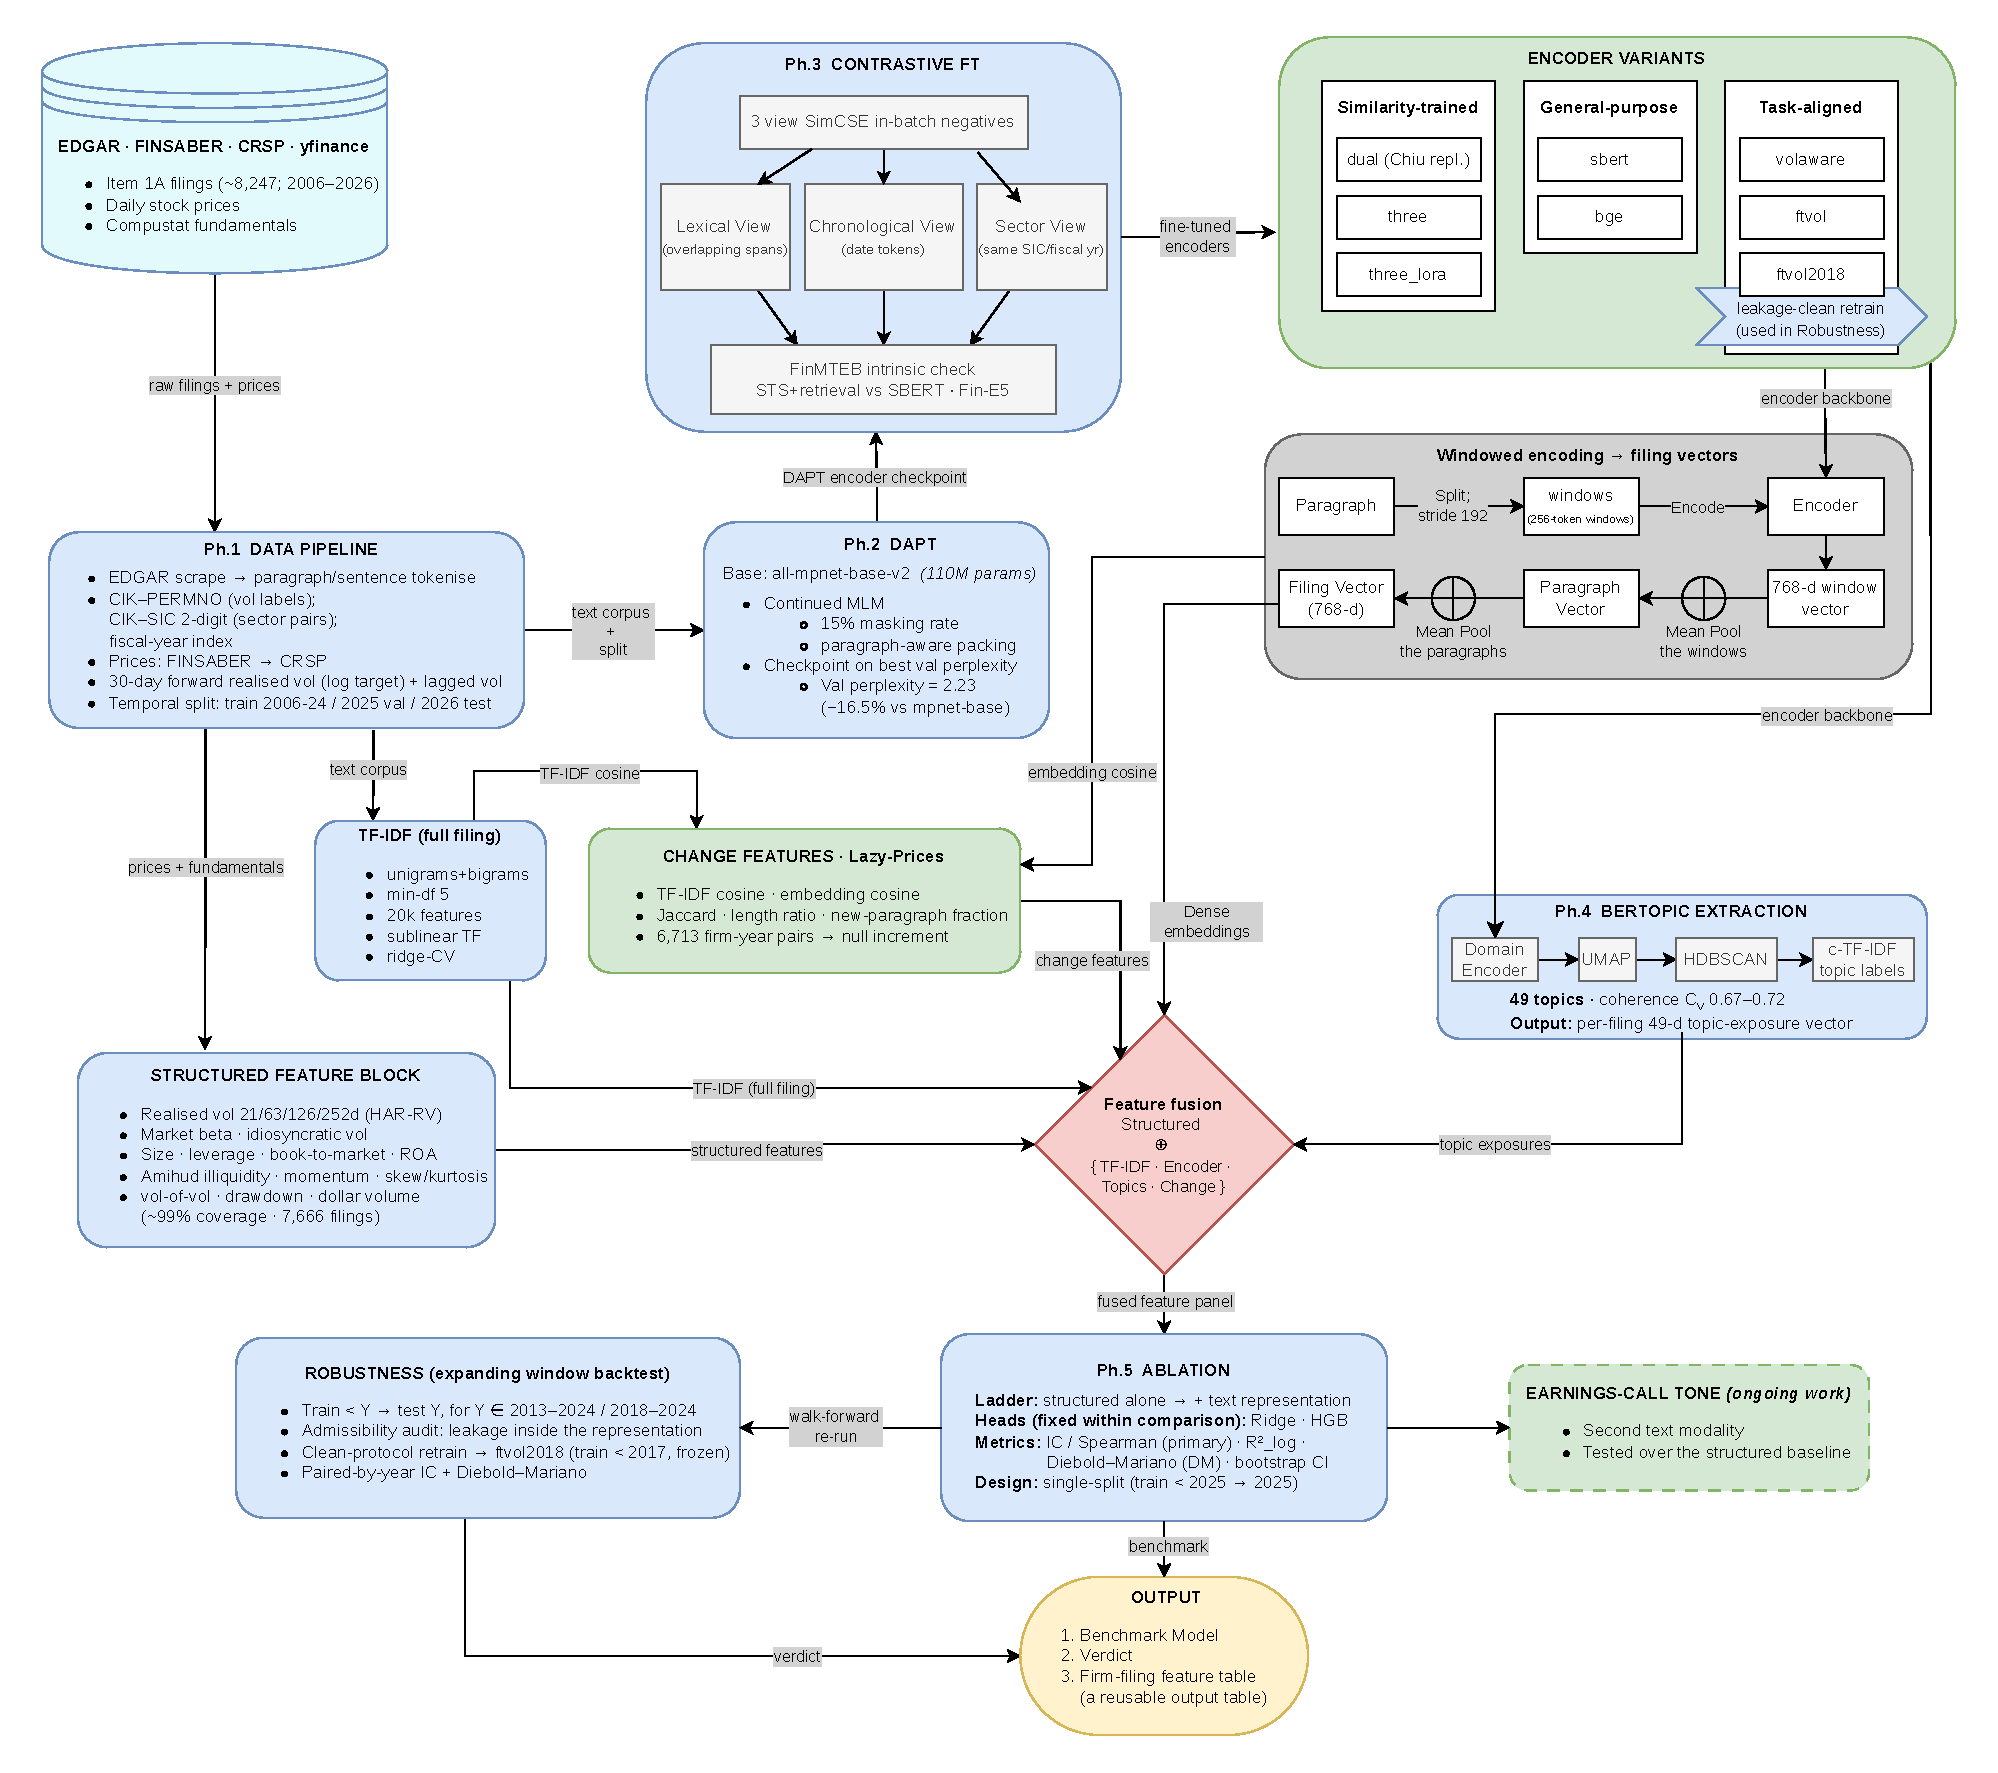
\includegraphics[width=\linewidth]{images/Dissertation_Flowchart.drawio.pdf}
    \caption{The finalised pipeline. Data and labels feed two parallel feature families: a structured financial block and a set of text representations (DAPT $\rightarrow$ three-view contrastive fine-tuning, additional and task-aligned encoders, windowed encoding, BERTopic, and disclosure-change features). All representations are fused in the ablation ladder under a fixed head, evaluated on the single forward split and then under an expanding-window backtest with an admissibility audit and a clean-protocol retrain.}
    \label{fig:pipeline}
\end{figure}

%==========================================================
\chapter{Methodology}
\label{sec:method}

Figure~\ref{fig:pipeline} shows the finalised pipeline that this chapter describes. Reading it from left to right, a data-and-label stage (Ph.1) assembles the Item~1A corpus, the volatility labels, and the temporal split, and feeds two parallel feature families. The first is a structured financial block of standard volatility predictors. The second is a set of text representations: a domain-adapted encoder (Ph.2, DAPT), its three-view contrastive variants (Ph.3), additional and task-aligned encoders, a windowed-encoding step that turns each filing into a dense vector, a BERTopic axis (Ph.4) that yields topic exposures, and a disclosure-change branch. The two families meet at the fusion step, where each text representation is added on top of the structured baseline and passed to a fixed prediction head (Ph.5, ablation). The resulting models are evaluated first on a single forward split, and then under an expanding-window backtest with an admissibility audit and a clean-protocol retrain, which together produce the defended benchmark and its verdict. The sections below follow this order: the problem and target (\S\ref{sec:target}), the data and the two feature families (\S\ref{sec:data} to \S\ref{sec:text}), and the evaluation protocol (\S\ref{sec:protocol}). Stages unchanged from the original design are described in full so the chapter stands alone; where the extended study altered or added a stage, the change is stated explicitly.

\section{Problem formulation and target}
\label{sec:target}
The task is to predict a firm's 30-day forward realised volatility from the text of its Item~1A ``Risk Factors'' disclosure and its structured characteristics. Volatility is the standard deviation of daily log returns over the 30 trading days strictly after the filing date, annualised by $\times\sqrt{252}$; the lagged measure uses the 30 trading days strictly before. The modelling target is $\log$ forward volatility, because volatility is approximately log-normal and strictly positive, and using the log everywhere keeps error metrics comparable across models.

Two metrics are reported throughout. The \textbf{information coefficient (IC)} is the within-year cross-sectional Spearman rank correlation between predicted and realised volatility; it answers whether the model ranked firms correctly from least to most volatile within a year. $\mathbf{R^2_{\log}}$ is the coefficient of determination on the log level. Ranking is the primary lens because the economic use of such a model is cross-sectional, while the level is dominated by market-wide conditions. Magnitudes must be judged against a persistence baseline, not against zero: Grinold and Kahn~\cite{grinold2000active} note that an IC of about 0.06 already implies a top-decile information ratio for \emph{return} forecasting, while Corsi~\cite{corsi2009simple} shows volatility is far more forecastable than returns, so within-year volatility ICs of 0.5--0.6 are the relevant range.

\section{Data and labels}
\label{sec:data}
The universe is the S\&P~500, including delisted firms to avoid survivorship bias. The text corpus is one Item~1A section per filing, approximately 8{,}247 filings spanning roughly 2006 to 2026; the master feature table has one row per filing (about 8{,}105 rows), keyed by ticker and fiscal year. Filing dates are indexed from EDGAR, and firm identifiers are linked across the SEC and finance worlds: \textbf{CIK--PERMNO} for volatility-label assignment, \textbf{CIK--SIC} (2-digit) via the EDGAR submissions API for sector-view pair construction, and a fiscal-year index aligning filing dates to return windows. Daily prices come from two sources in priority order: the FINSABER S\&P~500 price file (2000--2024, including delisted names), and WRDS CRSP daily returns for 2025.

The temporal split, used identically by every stage, is: training on filings dated before 2025-01-01 (about 7{,}353 filings), validation on 2025 filings (406 filings, of which about 397 have complete labels), and a held-out 2026 test year whose forward windows had not closed at the time of the experiments. All model selection and fitting uses the training years only. As a reusable research artefact, and to keep the representation module separable from the prediction head, a firm-filing feature table is assembled that joins the identifiers, the dense and topic representations, and the lagged and forward volatility labels into one ML-ready record (schema in Appendix~\ref{app:schema}).

\subsection{The structured feature block}
\label{sec:struct}
The structured block contains the standard cross-sectional volatility predictors, each grounded in the asset-pricing literature: realised volatility at horizons of 21, 63, 126 and 252 trading days (the multi-horizon persistence of HAR-RV \cite{corsi2009simple}); market beta and idiosyncratic volatility \cite{ang2006cross}; firm size, leverage and book-to-market \cite{ang2006cross,fama1992cross}; Amihud illiquidity \cite{amihud2002illiquidity}; return skewness and kurtosis \cite{conrad2013ex} (kurtosis as an exploratory control); momentum \cite{ang2006cross}; and vol-of-vol, drawdown and dollar volume. Fundamentals (log market capitalisation, leverage, book-to-market, return on assets) come from Compustat. Coverage is approximately 99\% across 7{,}666 filings. Building this block involved no new modelling, only feature engineering, which is precisely the point: it is the baseline any volatility study should start from, and the one the original text-only pipeline omitted.

\section{Text-representation modules}
\label{sec:text}

\subsection{Domain-adaptive pretraining (DAPT)}
Following Gururangan et al.\ \cite{gururangan2020don}, the encoder was first adapted to financial-risk language by continued masked-language-model (MLM) training on the 10-K corpus. The base model is \texttt{all-mpnet-base-v2} rather than raw \texttt{microsoft/mpnet-base}, because the sentence-transformer variant already has useful sentence-level geometry; only the encoder (not the MLM head) is carried forward, so the trade-off is to reshape its token vocabulary toward financial risk while preserving that geometry. The main design decision was how to chunk long Item~1A prose (median around 7{,}000 words) into 512-token sequences. Two within-document, non-overlapping greedy packers in the RoBERTa DOC-SENTENCES family \cite{liu2019roberta} were built: a sentence-aware packer, and a paragraph-aware packer that never splits an individual risk factor. This choice is supported by RoBERTa's ablation and its replication under tighter compute by Geiping and Goldstein \cite{geiping2023cramming}, and by the domain precedents LEGAL-BERT \cite{chalkidis2020legal} and SEC-BERT \cite{loukas2022finer}. An A/B comparison on an identical validation set selected the paragraph-aware variant (validation perplexity 2.2278 against 2.2671), with the recorded caveat that the margin is small and partly confounded by the paragraph variant taking about 22\% more gradient steps at a fixed five epochs. Training used the standard recipe: 15\% masking, learning rate $2\times10^{-5}$, effective batch 32, five epochs with early stopping on validation perplexity, fp16, 512-token sequences. The selected checkpoint reduces validation perplexity by about 16.5\% relative to \texttt{microsoft/mpnet-base} (2.23 against 2.67).

\subsection{Three-view contrastive fine-tuning}
The post-DAPT encoder was fine-tuned with a SimCSE-style InfoNCE objective with in-batch negatives \cite{gao2021simcse}, extending the dual-view framework of Chiu et al.\ \cite{chiu2025financial}, which pairs 256-token risk paragraphs. Three positive-pair views were constructed: a \textbf{lexical} view (two overlapping spans of the same paragraph), a \textbf{chronological} view (the same firm's matched risk factor in adjacent years, requiring TF-IDF cosine at least 0.5), and a new \textbf{sector} view (paragraphs from different firms in the same 2-digit SIC industry and fiscal year). Numbers and dates are normalised to \texttt{[NUM]} and \texttt{[DATE]} tokens following SEC-BERT \cite{loukas2022finer}. The loss is InfoNCE at temperature 0.05 \cite{gao2021simcse} with label-aware false-negative masking on the sector label \cite{khosla2020supervised}, and the soft sector view is down-weighted by 0.5. Pairs are built from the training split only. Three encoders were trained: \texttt{dual} (lexical + chronological, a replication of Chiu et al.), \texttt{three} (adding the sector view, full fine-tuning), and \texttt{three\_lora} (the sector variant with LoRA adapters, $r=16$ \cite{hu2022lora}). Each encoder was also scored intrinsically on the FinMTEB STS and retrieval sub-tasks \cite{tang-yang-2025-finmteb}, and the intrinsic scores are reported in Appendix~\ref{app:eval-tables}. They show the expected pattern: DAPT improves in-domain semantic similarity but damages retrieval geometry, which is the known anisotropy of raw MLM embeddings, and contrastive fine-tuning repairs it. A diagnosis of the sector view found that its random within-industry pairing produced many near-unrelated pairs. These pairs blurred the embedding geometry under full fine-tuning but were contained under LoRA.

\subsection{Additional and task-aligned encoders}
To make the encoder comparison exhaustive, three further encoders were added to the grid beyond the contrastive family. \texttt{sbert} is the off-the-shelf SBERT sentence transformer \cite{reimers2019sentence}, specifically the \texttt{all-mpnet-base-v2} checkpoint\footnote{\url{https://huggingface.co/sentence-transformers/all-mpnet-base-v2}} with no further adaptation. \texttt{bge} is BAAI's BGE model \cite{xiao2023cpack}, specifically the \texttt{bge-base-en-v1.5} checkpoint\footnote{\url{https://huggingface.co/BAAI/bge-base-en-v1.5}}, a modern strong general-purpose embedder included to address the objection that the original encoders were simply not good enough. Two \emph{task-aligned} encoders test whether aligning the objective with the target closes the gap. \texttt{volaware} is a contrastive encoder whose positive pairs are paragraphs from firms in the same within-year forward-volatility decile. \texttt{ftvol} is fine-tuned end-to-end on the volatility regression target itself, following the task-supervised precedents \cite{qin2019you,yang2020html}. A leakage-clean retrain of \texttt{ftvol}, called \texttt{ftvol2018}, is introduced in Section~\ref{sec:results-robust}.

\subsection{Windowed encoding}
\label{sec:windowed}
TF-IDF ingests the full filing by construction, so the encoders are given the same complete input through a windowed encoding step. Each long paragraph is split into overlapping 256-token windows with a stride of 192 tokens, every window is encoded, and the resulting window vectors are mean-pooled to a 768-dimensional paragraph vector before the usual paragraph-to-filing pooling. This produced 462{,}590 windows over 176{,}616 paragraphs in total. Segment-encode-pool is the established treatment of documents that exceed a transformer's context window \cite{beltagy2020longformer}, with the financial-NLP precedent of hierarchical transcript encoding \cite{yang2020html} and the 256-token paragraph unit of Chiu et al.\ \cite{chiu2025financial}.

\subsection{BERTopic topic extraction}
To provide the explanatory axis, BERTopic \cite{grootendorst2022bertopic} was fitted on the training paragraphs of each encoder's embedding space, with UMAP (15 neighbours, 5 components, cosine metric), then HDBSCAN (minimum cluster size 200), and a class-based TF-IDF topic representation reduced to 49 topics. The model is fitted on training documents only and applied to validation and test documents, so no held-out text shapes the topic space. Each filing receives a 49-dimensional topic-exposure vector (the fraction of its paragraphs assigned to each topic). Topic coherence ($C_V$) sits between 0.67 and 0.72 across encoders. The DAPT-only backend was excluded because its anisotropic embeddings prevent UMAP from converging.

\section{Evaluation protocol}
\label{sec:protocol}
Every condition is evaluated on the same data: one row per firm and filing year, so that models are always compared on identical inputs. Each condition is built by starting from the structured feature block and, where relevant, adding one text representation on top (TF-IDF, an encoder embedding, topic exposures, change features, or a combination of these). This step-by-step design is referred to as an ablation ladder, because each rung adds exactly one feature block to the structured baseline, and the resulting IC increment can be attributed to that one addition. Because the quantity of interest is a small increment on a strong baseline, three rules ensure that every comparison isolates exactly one difference.

\emph{First}, the prediction head is held fixed within every comparison. When the model class and the feature set change at once, credit assignment is arbitrary \cite{lipton2019troubling}, so both a ridge regression and a gradient-boosted tree (HGB) are reported for every condition, and increments are always quoted between same-head arms. \emph{Second}, every text representation receives the full text, via the windowed encoding of \S\ref{sec:windowed}, so a comparison between representations is not a comparison between the amounts of text each was allowed to read. \emph{Third}, statistical comparisons are paired: within each evaluation year the models predict the same firms, so per-year ICs are compared as matched pairs across years, and per-firm squared errors are compared by Diebold--Mariano tests \cite{diebold1995comparing}. The robustness extension of Section~\ref{sec:results-robust} adds the expanding-window (walk-forward) backtest that is standard for financial prediction \cite{de2018advances}.

\section{Compute used}
\label{sec:compute}
All training and evaluation ran on the University of Edinburgh's Teaching cluster under SLURM, using a different GPU configuration for each stage's memory and throughput needs. Domain-adaptive pretraining, the three contrastive fine-tuning runs, and the FinMTEB intrinsic evaluation ran on a full NVIDIA RTX~A6000; the FinMTEB evaluation alone took about 49 minutes on this GPU. The vol-aware contrastive encoder (\texttt{volaware}) used a full NVIDIA H200. Lighter single-GPU jobs, namely the supervised \texttt{ftvol} fine-tune, the full-text windowed re-encoding of the corpus, and the BERTopic fit, ran on an H200 partitioned as a smaller 1g.18gb MIG slice, while the more demanding clean-protocol \texttt{ftvol2018} retrain (20 epochs, batch size 128) used a larger 3g.71gb MIG slice of the same card. The Phase~5 ablation and the walk-forward backtest work on pre-computed feature vectors rather than raw text, so these ran on CPU-only nodes with no GPU allocation.

GPU jobs were budgeted up to 48 hours of wall-clock time, with a shorter 12-hour budget for the lighter FinMTEB and encoding jobs. BERTopic's UMAP and HDBSCAN clustering step is CPU-bound even when scheduled on a GPU node: an earlier attempt to fit UMAP over the DAPT-only embedding space was terminated after roughly ten hours without converging, which is the practical reason the DAPT-only backend was excluded from BERTopic in Section~\ref{sec:text}.

\section{Responsible research including ethics}
All data are sourced from publicly available, regulatory-mandated SEC filings (EDGAR) and aggregated market price feeds (CRSP, FINSABER, yfinance). No personal data, human subjects, or proprietary datasets are used, and no informed consent or IRB review is required. CRSP data are accessed exclusively through WRDS under the University's institutional licence and are not redistributed or retained beyond the project period.

%==========================================================
\chapter{Results}
\label{sec:results}

The primary results (\S\ref{sec:results-primary}) use the single-split design of the original pipeline (train before 2025, evaluate on 2025), which is the design most comparable to the literature. The robustness extension (\S\ref{sec:results-robust}) moves to walk-forward backtests and to an audit of the encoders' own training provenance. Sections~\ref{sec:results-change} and~\ref{sec:results-calls} cover the disclosure-change and earnings-call branches, and \S\ref{sec:results-synth} synthesises the verdict.

\section{How to read the tables}
Every results table uses these columns. \textbf{IC} is the within-year cross-sectional Spearman rank correlation (the primary metric). \textbf{95\% CI} is the bootstrap confidence interval on that single-year IC; with $n=393$ firms the interval spans roughly $\pm 0.06$, which is why single-year differences of 0.01--0.02 can never be conclusive on their own. $\mathbf{R^2_{\log}}$ is the coefficient of determination on the log level. \textbf{DM $p$} is the $p$-value of a Diebold--Mariano test \cite{diebold1995comparing} comparing the row's squared errors against the reference on the same firms. Condition names state the feature blocks and the head in brackets, so \texttt{struct+tfidf [sparse]} is structured features plus the TF-IDF block under the sparse ridge head.

\section{Primary results}
\label{sec:results-primary}

\subsection{Anchor results}
The baseline tiers (Table~\ref{tab:anchor}) are naive persistence, structured features under both heads, TF-IDF plus lagged volatility, and the defended model (structured plus TF-IDF). The TF-IDF vectoriser follows the standard strong lexical baseline \cite{kogan2009predicting,loughran2011liability}: English stop words removed, unigrams and bigrams, minimum document frequency 5, 20{,}000 features, sublinear term frequency, ridge penalty selected by cross-validation.

\begin{table}[h]
\centering
\footnotesize
\caption{Primary single-split results (train $<$ 2025, evaluate on 2025). Reference for the DM column is \texttt{struct+tfidf [sparse]}.}
\label{tab:anchor}
\begin{tabular}{@{}L{5.2cm}ccccc@{}}
\toprule
\textbf{Condition} & \textbf{IC} & \textbf{95\% CI} & $\mathbf{R^2_{\log}}$ & \textbf{DM $p$} \\
\midrule
\texttt{lagged [hgb]}            & 0.457 & --            & $-0.130$ & -- \\
\texttt{structured [hgb]}        & 0.558 & [0.487, 0.628] & 0.094   & 0.001 \\
\texttt{structured [ridge]}      & 0.591 & [0.522, 0.659] & 0.175   & 0.000 \\
\texttt{tfidf+lag [sparse]}      & 0.541 & --            & 0.116   & -- \\
\textbf{\texttt{struct+tfidf [sparse]}} & \textbf{0.603} & [0.534, 0.670] & \textbf{0.226} & reference \\
\bottomrule
\end{tabular}
\end{table}

Three statements summarise the table. First, the structured baseline alone beats the entire original text-only pipeline: 0.591 against the TF-IDF-plus-lagged floor of 0.541. The standard quantitative characteristics rank firm volatility better than any text-only method, which retroactively explains why the original pipeline's comparisons were all fought below this level. Second, text on top of the structured baseline adds: \texttt{struct+tfidf} reaches 0.603 IC and raises $R^2_{\log}$ from 0.175 to 0.226, and the Diebold--Mariano test says this accuracy gain is highly significant. Third, the IC increment ($+0.012$ on this single year) is inside the single-year confidence interval, which is exactly why Section~\ref{sec:results-robust} moves to multi-year paired tests before claiming anything about it.

\subsection{The encoder grid}
Table~\ref{tab:encgrid} scores every encoder under both heads with the full-text windowed inputs of \S\ref{sec:windowed}. The pattern is clean. The generic semantic encoders (\texttt{dual}, \texttt{sbert}, \texttt{bge}) sit at or below the no-text structured baseline and are significantly less accurate than \texttt{struct+tfidf} under a Diebold--Mariano test in at least one head. The inclusion of \texttt{bge} settles the ``you never tried a strong modern embedder'' objection: it loses too, even with the full text delivered through the windowed protocol. This direction has independent support, since FinMTEB reports that bag-of-words representations outperform dense embedding models on financial semantic-similarity tasks \cite{tang-yang-2025-finmteb}. The only encoders that reach statistical parity with the count model are the two trained on the volatility task itself, \texttt{ftvol} and \texttt{volaware}: task alignment, not model modernity, closes the gap. None of the parity rows beats the reference, and the kitchen-sink fusion of every representation at once also fails to beat it.

\begin{table}[h]
\centering
\footnotesize
\caption{Encoder grid (single-split 2025), full-text windowed inputs. Reference for the DM column is \texttt{struct+tfidf [sparse]}.}
\label{tab:encgrid}
\begin{tabular}{@{}L{6.6cm}cccc@{}}
\toprule
\textbf{Condition} & \textbf{IC} & \textbf{95\% CI} & $\mathbf{R^2_{\log}}$ & \textbf{DM $p$} \\
\midrule
\texttt{struct+enc[dual] [ridge]}      & 0.582 & [0.509, 0.652] & 0.162 & 0.013 \\
\texttt{struct+enc[dual] [hgb]}        & 0.582 & [0.511, 0.651] & 0.160 & 0.051 \\
\texttt{struct+enc[sbert] [ridge]}     & 0.562 & [0.482, 0.636] & 0.017 & 0.000 \\
\texttt{struct+enc[sbert] [hgb]}       & 0.591 & [0.521, 0.658] & 0.149 & 0.043 \\
\texttt{struct+enc[bge] [ridge]}       & 0.580 & [0.506, 0.649] & 0.093 & 0.000 \\
\texttt{struct+enc[bge] [hgb]}         & 0.584 & [0.512, 0.651] & 0.145 & 0.023 \\
\texttt{struct+enc[volaware] [ridge]}  & 0.587 & [0.514, 0.656] & 0.147 & 0.003 \\
\texttt{struct+enc[volaware] [hgb]}    & 0.597 & [0.530, 0.663] & 0.207 & 0.593 \\
\texttt{struct+enc[ftvol] [ridge]}     & 0.606 & [0.540, 0.672] & 0.185 & 0.207 \\
\texttt{struct+enc[ftvol] [hgb]}       & 0.598 & [0.529, 0.666] & 0.167 & 0.155 \\
\texttt{struct+enc[ftvol, topk\_risk] [hgb]} & 0.607 & [0.538, 0.677] & 0.194 & 0.454 \\
\texttt{struct+tfidf\_svd [ridge]}     & 0.594 & [0.526, 0.661] & 0.167 & 0.000 \\
\texttt{EVERYTHING svd+enc[ftvol]+chg [hgb]} & 0.608 & [0.542, 0.675] & 0.170 & 0.204 \\
\texttt{EVERYTHING tfidf+enc[ftvol]+chg [sparse]} & 0.590 & [0.525, 0.662] & 0.165 & 0.135 \\
\bottomrule
\end{tabular}
\end{table}

This grid also settles a question left open by the original pipeline. After the first, text-only ablation, it was suggested that a task-supervised encoder, trained directly on the volatility target, would outperform the other encoders. That encoder (\texttt{ftvol}) was built and tested here, and it reaches parity with the count model but does not beat it.

One caveat applies to this table and affects everything that follows in Section~\ref{sec:results-robust}. The parity rows come from encoders whose training data included volatility labels from before 2025, the exact period being evaluated. The \texttt{ftvol} checkpoint was also selected using its performance on the validation year itself. Both practices let information about the evaluation period leak into training, so these rows overstate what the encoder could do on genuinely unseen data. They are useful as exploratory evidence but should not be read as a fair result. Section~\ref{sec:results-robust} removes this leakage and reports what a task-aligned encoder can really do.

\section{The robustness extension}
\label{sec:results-robust}
Everything here goes beyond the original evaluation design, and is a deliberate methodological adaptation: the single-year comparison cannot statistically separate models 0.01 apart, and, more seriously, it cannot detect a class of leakage that turned out to be present.

\subsection{The expanding-window backtest}
The protocol is the standard walk-forward design for financial prediction \cite{de2018advances}. For each test year $Y$ from the start year to 2024, every model is trained on filings from years strictly before $Y$ and scored on year $Y$, exactly as a deployed model would have been. Two windows are reported, 2013--2024 and 2018--2024; the $t$-statistic is the mean yearly IC divided by its standard error across years, so it measures the consistency of the ranking skill.

\begin{table}[h]
\centering
\footnotesize
\caption{Expanding-window backtest: IC (and $t$-statistic across years).}
\label{tab:backtest}
\begin{tabular}{@{}L{5.2cm}cc@{}}
\toprule
\textbf{Condition} & \textbf{2018--2024 IC ($t$)} & \textbf{2013--2024 IC ($t$)} \\
\midrule
\texttt{lagged [hgb]}            & 0.456 (4.6) & 0.526 (8.3) \\
\texttt{structured [hgb]}        & 0.511 (5.0) & 0.584 (9.0) \\
\texttt{structured [ridge]}      & 0.546 (5.6) & 0.603 (9.9) \\
\texttt{tfidf+lag [sparse]}      & 0.499 (5.2) & 0.558 (9.3) \\
\textbf{\texttt{struct+tfidf [sparse]}} & \textbf{0.561 (5.9)} & \textbf{0.614 (10.4)} \\
\bottomrule
\end{tabular}
\end{table}

Paired across years against the fair \texttt{structured [ridge]} baseline, \texttt{struct+tfidf} adds $+0.016$ IC ($p=0.098$) on the seven-year window and $+0.011$ IC ($p=0.057$) on the twelve-year window. The text increment is small, positive in sign in both windows and in most individual years, and just short of the conventional significance threshold on twelve years of data; the structured baseline's own superiority over pure persistence is unambiguous ($+0.059$ IC over lagged, $p=0.007$). This is the honest shape of the headline result: a strong structured baseline, plus a small, consistent, statistically suggestive lexical text increment, with a much clearer text advantage on level accuracy than on ranking.

\subsection{The admissibility audit}
Before running encoder backtests, the training provenance of each encoder was checked against the backtest years. This check found that the two task-aligned encoders could not be legitimately backtested with their existing checkpoints. \texttt{ftvol} was trained on the volatility labels of all pre-2025 filings, and its best epoch was chosen using validation-year IC. \texttt{volaware}'s contrastive pairing used within-year forward-volatility deciles computed across all pre-2025 filings. Both practices mean the same checkpoint that would be tested on, say, 2018 had already seen 2018 labels during its own training. This is lookahead leakage, even though the downstream prediction head is trained cleanly on each backtest year. It is the same temporal-leakage failure mode the methodology literature warns about \cite{de2018advances}, but one level removed: the leak sits inside the text representation rather than inside the predictor. For the same reason, change features derived from these two encoders' embeddings are excluded from every backtest. As a result, the in-period parity of \texttt{ftvol} and \texttt{volaware} reported in Section~\ref{sec:results-primary} could be neither confirmed nor refuted by any backtest using the existing checkpoints, and a retrain under a clean protocol was required.

\subsection{The clean-protocol retrain and the final verdict}
The decisive experiment retrains the supervised encoder under a strict temporal cutoff. Training uses only filings from before 2017, the best epoch is chosen on 2017, and the resulting checkpoint is then frozen. Years 2018--2024 are never touched by the encoder in any way, which makes the 2018--2024 backtest admissible by construction. The retrained encoder (\texttt{ftvol2018}) is strong in-period, with a filing-level IC of 0.635 on its 2017 selection year from text alone, confirming that the supervised objective learns a real signal.

\begin{table}[h]
\centering
\footnotesize
\caption{Clean-protocol retrain: out-of-period backtest (2018--2024).}
\label{tab:clean}
\begin{tabular}{@{}L{5.6cm}ccc@{}}
\toprule
\textbf{Lane} & \textbf{mean IC} & \textbf{vs \texttt{struct+tfidf}} & \textbf{vs \texttt{structured [hgb]}} \\
\midrule
\texttt{struct+enc[ftvol2018] [ridge]} & 0.504 & $-0.057$ ($p=0.087$) & $-0.007$ ($p=0.83$) \\
\texttt{struct+enc[ftvol2018] [hgb]}   & 0.497 & $-0.064$ ($p=0.097$) & $-0.014$ ($p=0.64$) \\
\texttt{struct+tfidf [sparse]} (ref.)  & 0.561 & --                  & $+0.050$ ($p=0.11$) \\
\bottomrule
\end{tabular}
\end{table}

Out of period, the encoder collapses. Its embeddings add nothing over the structured features alone, since the difference is statistically zero, and it loses to the count model by about 0.06 IC. Combined with the encoder grid, this gives the verdict of the whole study: \textbf{no encoder configuration beats the count-based model under any admissible protocol.} The apparent parity of the original \texttt{ftvol} on the validation year is now explained. It came from training on all pre-2025 labels plus epoch selection on the evaluation year, and the clean protocol removes both of these advantages.

The result also carries a positive characterisation, which is the more interesting contribution. Task-aligned training closes the gap in-period, but that advantage does not survive forward transfer. The dense text-to-volatility mapping the encoder learns is era-specific: it captures the relationship between the training era's risk vocabulary and volatility, and that relationship drifts over time. The TF-IDF lanes are not immune to drift because bag-of-words is a better representation in any single year. They are immune because the lexical features are transparent levels, and an annually refit linear head can re-weight them each year at negligible cost. This reading is consistent with the concept-drift framework \cite{lu2018learning} and with the time-varying text-return relationships documented on this disclosure section by Magner et al.\ \cite{magner2025decoding}.

One point about the comparison is worth noting: the frozen \texttt{ftvol2018} checkpoint is up to eight years older than the TF-IDF lanes, which are refit every year (see Limitations, Chapter~\ref{sec:discussion}). Even the one case with no staleness at all, the original \texttt{ftvol} evaluated on 2025, only ties with the count model rather than beating it, so this age gap is unlikely to change the verdict.

\section{Disclosure-change features (the Lazy-Prices branch)}
\label{sec:results-change}
Cohen, Malloy and Nguyen \cite{cohen2020lazy} showed that year-over-year changes in 10-K text predict returns. In their account, the alpha comes from investors under-reacting to the changes that do occur. Kravet and Muslu \cite{kravet2013textual} report the volatility-side analogue of this effect. This corpus shows a similar pattern of persistence, which a stale-text experiment quantifies directly. Roughly three quarters of the filings were re-paired with the adjacent year's risk text instead of their own, and the \texttt{struct+tfidf} validation IC was essentially unchanged (0.611 against 0.610). Year-stale risk text therefore predicts volatility almost exactly as well as current risk text. This means the text signal identified in Section~\ref{sec:results-primary} sits in the persistent \emph{level} of the risk language rather than in how recently it was written, which agrees with Campbell et al.\ \cite{campbell2014information}. This persistence sharpens the question for the rest of this section: if the level of risk language barely moves from year to year, do the small movements that do occur carry any additional information about volatility?

To test this, a set of change features was built for each consecutive firm-year pair, covering 6{,}713 firm-year pairs in total. The features are: TF-IDF cosine similarity between the two filings, embedding cosine similarity under the admissible encoders, Jaccard overlap of the text, the ratio of filing lengths, and the fraction of paragraphs in the later filing with no close match in the earlier one. These features pass a simple construction check: median lexical similarity dips visibly in fiscal 2020 (0.964, against roughly 0.976 in normal years), which is exactly where the COVID-19 rewrite of risk sections should show up.

\begin{table}[h]
\centering
\footnotesize
\caption{Disclosure-change features: expanding-window backtest.}
\label{tab:change}
\begin{tabular}{@{}L{5.6cm}cc@{}}
\toprule
\textbf{Condition} & \textbf{2018--2024 IC ($t$)} & \textbf{2013--2024 IC ($t$)} \\
\midrule
\texttt{struct+change [hgb]}         & 0.492 (4.8) & 0.575 (8.7) \\
\texttt{struct+tfidf+change [sparse]} & 0.550 (5.9) & 0.606 (10.5) \\
\texttt{struct+tfidf [sparse]} (ref.) & 0.561 (5.9) & 0.614 (10.4) \\
\bottomrule
\end{tabular}
\end{table}

The verdict is null. Adding change features to the count model performs slightly worse than the count model alone on both windows (paired differences of $-0.011$ and $-0.007$, $p=0.37$ and $0.28$), and change features without TF-IDF perform worse than the structured baseline. Disclosure change, whether measured lexically or semantically, adds no incremental volatility signal beyond the level of the text. This null result is consistent with the source literature. The Lazy-Prices effect is specifically a \emph{returns} phenomenon, driven by investors under-reacting to changes in the text. For volatility, by contrast, the informative quantity is the level of risk language rather than its year-over-year shift.

\section{Earnings-call tone (ongoing)}
\label{sec:results-calls}
A second text modality, the earnings call, is being tested as an ongoing extension (Stage~C). Because the 2025 call collection postdated the 10-K filings, a filing-level test was not possible; the question was instead tested call-anchored (does call tone predict the 30-day volatility following the call?). Inside the full model (structured block plus tone under an HGB head, leave-one-quarter-out), tone adds $+0.039$ IC over structured alone, roughly the same increment that 10-K text adds, though the status is suggestive and unconfirmed ($n=152$ calls, a single 2024--2025 regime). The methodological lesson worth keeping is that a feature can add nothing on its own yet add real value in combination, so incremental tests must be run inside the full model. Full detail and the planned confirmation collection are in Appendix~\ref{app:calls}.

\section{Synthesis: the defended benchmark}
\label{sec:results-synth}
The final model of the study is the structured feature block plus full-text TF-IDF under a sparse ridge head. Its performance is strong and consistent: a mean IC of 0.614 ($t=10.4$) over the twelve-year expanding-window backtest, and an $R^2_{\log}$ of 0.226 on the 2025 validation year. It also carries a small text increment over the fair structured baseline of $+0.011$ IC ($p=0.057$), together with a decisively significant gain in accuracy.

This model was tested against every challenger fielded across the study: two prediction heads, eight text representations, three pooling schemes, five encoders (including a modern general-purpose embedder and two task-supervised ones), topic exposures, change features, and full fusion models. All of these comparisons were run under leakage-audited conditions, extending even to the training provenance of the encoders themselves, and the defended model beat every one of them.

The underlying explanation is straightforward. The volatility signal in Item~1A text is lexical-level, persistent, and can be captured by a simple count-based representation. Task-aligned encoders can learn this signal within their training period, but the mapping they learn is specific to that period and does not transfer forward in time. Lexical features do not have this problem, because they are refit every year and so stay current by construction.

%==========================================================
\chapter{Discussion and Conclusions}
\label{sec:discussion}

\textbf{Contributions.} This study makes four contributions, and each rests on a broad, carefully controlled evaluation rather than a single comparison. First, it turns the original one-year finding, that TF-IDF beats every learned encoder, into a defended benchmark: the same conclusion now stands up against a wide grid of alternatives across twelve years of walk-forward backtests. That grid is deliberately exhaustive, spanning non-text baselines (persistence, structured financial features), simple-text baselines (TF-IDF and its Loughran--McDonald-calibrated reading), and representation baselines (SBERT, BGE, the contrastive encoders, and topic exposures), all scored under the same incremental-value test and the same fixed prediction head. Second, the study explains \emph{why} the count-based model wins. The volatility signal in risk-factor text is lexical and persistent, and although a task-aligned encoder can learn this signal within its own training period, the mapping it learns is specific to that period and does not carry over to later years; to our knowledge, this is the first time a volatility-supervised text encoder has been tested this honestly outside its training period. Third, the study establishes a persistence finding: risk-factor text from the previous year predicts volatility almost as well as the current year's text. Fourth, it reports a null result with an explanation, namely that changes in disclosure text do not improve volatility prediction, and the contrast with the Lazy-Prices literature on returns explains why. Alongside these findings, the study produces a reusable firm-filing feature table as a standalone deliverable, so that the underlying representations can be reused directly without repeating the full pipeline.

\textbf{Limitations.} The results have four main limitations, none of which undermines the headline finding but each of which bounds how far it can be pushed. The text increment on ranking accuracy is small and, while positive and consistent across most years, its statistical significance is still borderline ($p=0.057$ over twelve years); this is best read as a trend that more evaluation years will sharpen rather than a result that further data would overturn. The clean-protocol retrain compares a frozen 2018 encoder against text representations that are refit every year, which gives the encoder an unavoidable staleness disadvantage of one to eight years; retraining the encoder inside every backtest window would remove this disadvantage but requires twelve separate GPU fine-tunes, which was outside the scope of the current study. The level-based $R^2$ metric is noisy in individual backtest years and occasionally negative, which is why the ranking-based information coefficient is used as the primary and more reliable measure throughout. Finally, the earnings-call tone result is an early-stage pilot based on a small sample from a single period, and should be read as suggestive rather than confirmed.

\textbf{Future work.} Four directions follow directly from these limitations. The planned confirmation collection of pre-filing 2025 earnings calls will test whether the call-tone result holds up as a genuine, forward-looking signal rather than a pilot artefact. As more evaluation years accumulate, the text increment over the structured baseline can be re-tested to see whether it crosses the conventional significance threshold, which its current trend across windows suggests it will. A longer-term extension would retrain the task-aligned encoder inside each backtest window, removing the staleness handicap entirely and testing directly whether more frequent retraining can close the out-of-period gap, or whether the era-specific mapping problem is more fundamental than retraining frequency can fix. Finally, benchmarking the \texttt{dual} replication directly against Chiu et al.\ \cite{chiu2025financial} on their own retrieval task, rather than only on the volatility task used here, would clarify how much of the encoder grid's performance reflects the retrieval-style contrastive objective itself.

%==========================================================
\chapter{Research Plan, Milestones, and Deliverables}
\label{sec:plan}

The original six-phase plan (Phases~1--6) has been delivered, and the extended study added four further stages of work: the structured baseline and reframing, the robustness backtest with its admissibility audit and clean-protocol retrain, the disclosure-change branch, and the earnings-call pilot. Figure~\ref{fig:gantt} shows the programme as delivered, with the remaining work (the pre-filing 2025 call-confirmation collection and final write-up) marked as a contingency. Extended-study dates are indicative. Tables~\ref{tab:milestones} and~\ref{tab:deliverables} give the milestones and deliverables, updated to reflect completion and the reusable feature-table deliverable.

\begin{figure}[htbp]
\centering
\resizebox{\linewidth}{!}{%
\begin{ganttchart}[
    y unit title=0.4cm,
    y unit chart=0.5cm,
    vgrid, hgrid,
    x unit=1.1mm,
    time slot format=isodate-yearmonth,
    title/.append style={draw=none, fill=accentblue},
    title label font=\sffamily\bfseries\color{white},
    bar/.append style={draw=none, fill=mainblue},
    bar height=.6,
    bar label font=\normalsize\color{black!50},
    link/.style={-stealth, thick, black!65}
]{2025-05}{2026-08}
   \gantttitlecalendar{year, month=shortname}\\
   \ganttbar{Ph.1 Data pipeline}{2025-05}{2025-05} \\
   \ganttbar{Ph.2 DAPT}{2025-05}{2025-06} \\
   \ganttbar{Ph.3 Contrastive FT}{2025-06}{2025-06} \\
   \ganttbar{Ph.4 BERTopic}{2025-06}{2025-07} \\
   \ganttbar{Ph.5 Original ablation}{2025-07}{2025-07} \\
   \ganttbar{Structured baseline + reframing}{2025-08}{2025-11} \\
   \ganttbar{Robustness backtest + audit}{2025-12}{2026-03} \\
   \ganttbar{Change-features branch}{2026-02}{2026-04} \\
   \ganttbar{Earnings-call pilot (ongoing)}{2026-04}{2026-07} \\
   \ganttbar[bar/.append style={fill=orange!75, draw=none}]{Call confirmation + final submission}{2026-07}{2026-08} \\
   \ganttbar[bar/.append style={fill=mainblue!30, draw=none}]{Write-up (continuous)}{2025-05}{2026-08}
\end{ganttchart}%
}
\caption{Programme as delivered.
\textcolor{mainblue}{\rule[0.4ex]{1.2em}{0.7em}}~completed stage;\enspace
\textcolor{orange!75}{\rule[0.4ex]{1.2em}{0.7em}}~remaining work;\enspace
\textcolor{mainblue!30}{\rule[0.4ex]{1.2em}{0.7em}}~continuous write-up. Extended-study dates are indicative.}
\label{fig:gantt}
\end{figure}

\begin{table}[htbp]
\centering
\begin{tabular}{@{}cL{9cm}c@{}}
\toprule
\textbf{Milestone} & \textbf{Description} & \textbf{Status} \\
\midrule
$M_1$ & Clean corpus, temporal split indices, volatility labels & Done \\
$M_2$ & Domain-adapted encoder + perplexity benchmarks & Done \\
$M_3$ & Contrastive encoders + FinMTEB intrinsic scores & Done \\
$M_4$ & BERTopic coherence + per-filing topic-feature matrix & Done \\
$M_5$ & Original ablation results + forecasting metrics & Done \\
$M_6$ & Structured baseline + reframed incremental-value ablation & Done \\
$M_7$ & Walk-forward backtest, admissibility audit, clean-protocol verdict & Done \\
$M_8$ & Disclosure-change + persistence analysis & Done \\
$M_9$ & Earnings-call confirmation + final report & Remaining \\
\bottomrule
\end{tabular}
\caption{Project milestones.}
\label{tab:milestones}
\end{table}

\begin{table}[htbp]
\centering
\begin{tabular}{@{}cL{9cm}c@{}}
\toprule
\textbf{Deliverable} & \textbf{Description} & \textbf{Status} \\
\midrule
$D_1$ & Domain-adapted encoder (DAPT checkpoint) & Done \\
$D_2$ & Contrastive fine-tuned encoders + FinMTEB evaluation & Done \\
$D_3$ & BERTopic topic analysis + per-filing topic-feature matrix & Done \\
$D_4$ & Structured feature block + reusable firm-filing feature table & Done \\
$D_5$ & Full ablation + walk-forward backtest results & Done \\
$D_6$ & Disclosure-change feature analysis & Done \\
$D_7$ & Earnings-call pilot + final report + reproducible codebase & Remaining \\
\bottomrule
\end{tabular}
\caption{Project deliverables.}
\label{tab:deliverables}
\end{table}

%-------------------- References -------------------------
\bibliographystyle{unsrt}
\bibliography{main}


% You may delete everything from \appendix up to \end{document} if you don't need it.
\appendix

\chapter{Supplementary evaluation tables}
\label{app:eval-tables}
The main-text tables (Chapter~\ref{sec:results}) report the load-bearing rows of a larger evaluation grid; this appendix gives the remaining detail. Table~\ref{tab:finmteb} reports the FinMTEB intrinsic scores referenced in Section~\ref{sec:text}, and Table~\ref{tab:pooling} reports the additional pooling-scheme variants run as part of the encoder grid of Section~\ref{sec:results-primary}. The full per-year backtest series behind each $t$-statistic in Section~\ref{sec:results-robust} are held in the project's Phase~5 result logs and are not reproduced here.

\begin{table}[h]
\centering
\footnotesize
\caption{FinMTEB intrinsic evaluation (zero-shot). STS is mean Spearman $\rho$ over two English STS tasks; retrieval is mean NDCG@10 over ten English retrieval tasks.}
\label{tab:finmteb}
\begin{tabular}{@{}lcc@{}}
\toprule
\textbf{Model} & \textbf{STS mean ($\rho$)} & \textbf{Retrieval mean (NDCG@10)} \\
\midrule
\texttt{sbert} & 0.312 & 0.605 \\
\texttt{dapt} & 0.465 & 0.326 \\
\texttt{dual} & 0.406 & 0.497 \\
\texttt{three} & 0.337 & 0.419 \\
\texttt{three\_lora} & 0.410 & 0.502 \\
\bottomrule
\end{tabular}
\end{table}

DAPT is the strongest model on STS (0.465) but the weakest on retrieval (0.326), which is the known anisotropy of raw MLM embeddings referenced in Section~\ref{sec:text}. Both contrastive encoders recover most of this retrieval loss, and \texttt{three\_lora} is the strongest of the three encoders on both axes. SBERT still leads overall retrieval, which is expected rather than a shortfall: it was trained on over a billion general-domain pairs, and FinMTEB's retrieval tasks (generic finance question answering, 10-K and news retrieval) are out of distribution for an encoder specialised on Item~1A risk paragraphs. FinMTEB is treated throughout as a supporting intrinsic check rather than the decisive metric; that role belongs to the downstream volatility evaluation of Chapter~\ref{sec:results}.

\begin{table}[h]
\centering
\footnotesize
\caption{Supplementary pooling-scheme variants, single-split 2025. Reference for the DM column is \texttt{struct+tfidf [sparse]}.}
\label{tab:pooling}
\begin{tabular}{@{}L{6.6cm}ccc@{}}
\toprule
\textbf{Condition} & \textbf{IC} & $\mathbf{R^2_{\log}}$ & \textbf{DM $p$} \\
\midrule
\texttt{struct+tfidf\_svd [hgb]} & 0.569 & 0.167 & 0.123 \\
\texttt{struct+enc[ftvol, risk\_weighted] [hgb]} & 0.604 & 0.185 & 0.324 \\
\texttt{struct+enc[dual/sbert, risk\_weighted/topk\_risk]} & 0.573--0.578 & 0.145--0.172 & $\leq$0.128 \\
\texttt{struct+enc[volaware, risk\_weighted/topk\_risk] [hgb]} & 0.586--0.593 & 0.180--0.203 & $\geq$0.165 \\
\bottomrule
\end{tabular}
\end{table}

The two mean-pooling and risk-weighted pooling variants shown here sit inside the same range as their mean-pooled counterparts in Table~\ref{tab:encgrid}, so the choice of pooling scheme does not change the conclusion of Section~\ref{sec:results-primary}: no pooling variant of any encoder beats the reference.

\chapter{Structured feature definitions}
\label{app:features}
The structured block (\S\ref{sec:struct}) comprises: realised volatility at 21/63/126/252 trading-day horizons (HAR-RV \cite{corsi2009simple}); market beta and idiosyncratic volatility relative to a factor model \cite{ang2006cross}; log market capitalisation (size), leverage, book-to-market \cite{fama1992cross,ang2006cross} and return on assets (Compustat); Amihud illiquidity as $|R|/$dollar-volume \cite{amihud2002illiquidity}; return skewness and kurtosis \cite{conrad2013ex} (kurtosis exploratory); past-12-month momentum \cite{ang2006cross}; and vol-of-vol, drawdown and dollar volume. Coverage is approximately 99\% across 7{,}666 filings.

\chapter{Training recipes and hyperparameters}
\label{app:recipes}
\emph{DAPT:} \texttt{all-mpnet-base-v2}; continued MLM at 15\% masking; learning rate $2\times10^{-5}$; effective batch 32; five epochs; early stopping on validation perplexity; fp16; 512-token, paragraph-aware, non-overlapping packing. \emph{Contrastive:} SimCSE-style InfoNCE, in-batch negatives, temperature 0.05; three views with the soft sector view down-weighted 0.5; label-aware false-negative masking on the 2-digit SIC label; \texttt{[NUM]}/\texttt{[DATE]} normalisation; 256-token paragraphs; LoRA rank 16 for \texttt{three\_lora}. \emph{Windowed encoding:} 256-token windows, stride 192, mean-pool to a 768-d paragraph vector; 462{,}590 windows over 176{,}616 paragraphs. \emph{BERTopic:} UMAP (15 neighbours, 5 components, cosine) $\rightarrow$ HDBSCAN (minimum cluster size 200) $\rightarrow$ class-based TF-IDF, 49 topics. \emph{Backtest:} expanding window, test years 2013--2024 and 2018--2024; clean-protocol retrain (\texttt{ftvol2018}) trained on years before 2017, epoch-selected on 2017, then frozen.

\chapter{Firm-filing feature-table schema}
\label{app:schema}
The reusable deliverable ($D_4$) is a firm-filing table, one row per filing: \texttt{CIK} (EDGAR), \texttt{PERMNO} (CRSP CCM linkage), \texttt{filing\_date} (EDGAR submissions API), \texttt{SIC2} (2-digit industry), the dense risk embedding (768-d, from the contrastive encoder), the topic-exposure vector (49-d, from BERTopic), \texttt{lagged\_vol\_30d} (CRSP), and \texttt{fwd\_vol\_30d} (the label; CRSP with a yfinance fallback for 2025--2026). The first four columns are identifiers, the next two are produced by the NLP pipeline, and the last two are financial labels, so one row is a self-contained record for reproducing or extending the experiments.

\chapter{Citation verification}
\label{app:citations}
All numeric and design-choice citations were verified against source PDFs across a four-round pass (recorded in \texttt{Literature\_agent\_study\_extended.md}). Two bibliographic housekeeping items are noted for completeness: the Grinold and Kahn edition year (1999 vs 2000) and the Diebold and Mariano 1995-original-vs-2002-reprint choice (the 1995 original is used here). Momentum is cited through Ang et al.\ \cite{ang2006cross}, where it appears as a standard control, rather than through Jegadeesh and Titman (1993), which could not be accessed.

\chapter{Earnings-call (Stage~C) pilot detail}
\label{app:calls}
The 2025 call collection postdated the 10-K filings, so a filing-level test was not possible; the question was tested call-anchored. A first crude test (tone against persistence, linearly) found nothing. Re-tested inside the full model (structured block plus tone under an HGB head, leave-one-quarter-out), tone adds $+0.039$ IC over structured alone (0.594 against 0.555), roughly the increment that 10-K text adds. The status is suggestive and unconfirmed ($n=152$ calls, a single 2024--2025 regime); a confirmation collection of the 406 pre-filing 2025 calls is specified in the project's call-collection specification document and remains pending. The task-supervised earnings-call precedents are Qin and Yang \cite{qin2019you}, Yang et al.\ (HTML) \cite{yang2020html}, and Sawhney et al.\ (VolTAGE) \cite{sawhney2020voltage}.

\end{document}
